\documentclass{article}

\usepackage{amsmath}
\usepackage{tikz}
\usepackage{graphicx}

\newcommand\class[1]{\texttt{#1}}
\newcommand\method[1]{\texttt{#1}}
\newcommand\attribute[1]{\texttt{#1}}

\begin{document}

\title{
    INE5450 --- C for device drivers \\
    Discipline report
}
\author{
    Lucas Pereira Zarbato --- 11100890 \\
    Paulo César Pereira Júnior --- 11202906 \\
    Tiago Royer --- 12100776
}
\date{December 9, 2015}
\maketitle

\section{General description of the project}

In essence, our project is an ``automatic laser aimer''.
We built a structure with two stepper motors and an attached laser
that will receive images from a camera.
This image is processed by the Raspberry Pi,
which then orders the stepper motors to rotate in order to
make the attached laser point towards a special marker in real world.

The marker is shown in figure (TODO: Add figure here).
The exact dimensions of the marker are known;
therefore, given a picture with the marker,
we can compute the distance between the camera and the marker.
The library ArUco does these calculations;
it gives us back a point in $3D$ space,
with the camera being the origin (point $(0, 0, 0)$).

But the laser is not centered in the camera,
so we need to calibrate the program to know where the camera is
and what are its rotation axis.
Four measurements are enugh:
first, move the marker to the front of the laser and take two photos
(with varying distances from the laser in each photo).
These two photos gives two points in the space
in the line of sight of the laser;
thus, the center of the laser and these two points are collinear.

Now, rotate the laser horizontally by a fixed number of degrees
(we have chosen $10$)
and take two more photos.
These photos give another pair of points collinear with the center of the laser.
This information is enough to determine everything needed
(the center of the laser and the rotation axis);
the maths are in section~\ref{sec:math}.

With the laser calibrated,
we can now make it aim to the marker!
After each photo taken,
the program calculates how much each stepper motor must rotate
in order to make the laser point to the marker.
After some cycles,
the laser is aimed there.

\section{Software Engineering}

Our program modules:
\begin{itemize}
    \item \class{Aimer} class: once the measures of the axis are made,
there is a method in this function that creates a new thread that verify
every time the camera detects a marker and updates the laser position.
    \item \class{Ballistics} class: this one is responsible for computing
how much each stepper motor must rotate. It starts its computing with
4 measures: 2 measures for the first line, then we give a kwnown angle and
make 2 new measures for the second line. With this measures we can infer 
the 3 axis in witch the laser is placed.
    \item \class{LaserAimer} class: like the \class{Aimer} class, this class
creates a new thread in charge of controlling the motors each time the 
\class{Aimer} thread updates the position of the marker.
    \item \class{LaserCalibrator} class: this one is responsible for catching
the 4 measures of the markers from the user that is using the program and make
that measure public for other classes, like \class{Ballistics} that use this
information to compute the axis.
    \item \class{TargetDetector} class: this class has the function of
detecting the augmented reality marker and giving back this information.
It detects the marker using the Aruco library.
This is used in \class{Aimer}, \class{LaserCalibrator} for example.
    \item \class{Stepper} class: each instance of this class is in charge of
controlling the PWM (Pulse Width Modulation) for each motor and it
gives a frendlier interface to someone that want to use the motors,
with methods such as \method{step(int n)} that execute \texttt{n} steps,
forwards or backwards depending on the signal of \texttt{n}
    \item math functions: generic mathematical subroutines that are mainly used in
\class{Ballistics} 
    \item main function: all the instances that are used in the program are
allocated here and are passed as parameters as it is needed. 
\end{itemize}

Softwares/Libraries used:
\begin{itemize}
    \item Aruco: Augmented reality library, it returns if detected the marker
and its 3D position.
    \item OpenCV: It's a open library for computer graphics otimizing as it can,
in multicore or in GPU. 
    \item WiringPi: This is a small library to control the GPIO pins in the
raspberry pi.
\end{itemize}

\section{Hardware Engineering}

\begin{figure}[h!]
    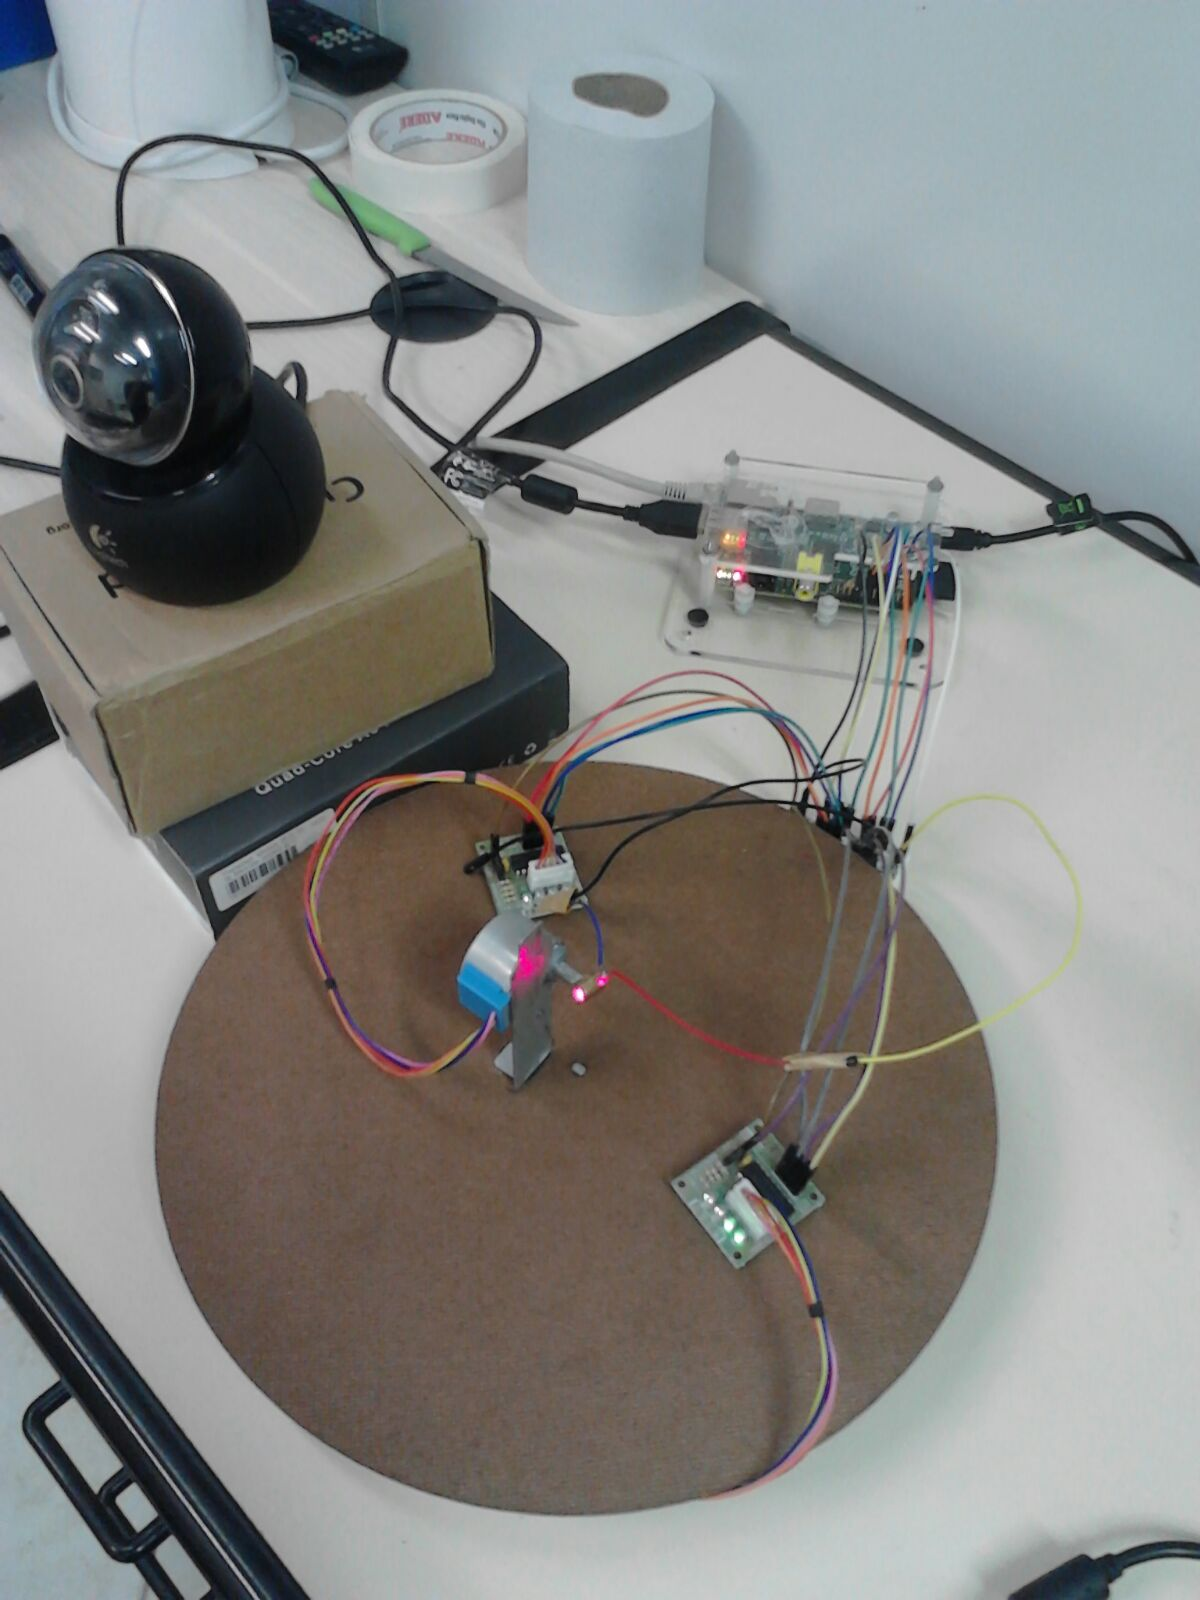
\includegraphics[scale=0.2]{imgs/hardware.jpg}
    \caption{The complete structure}
    \label{fig:img1}
\end{figure}

\section{Mathematics involved}
\label{sec:math}

This section describes the mathematics behind the \class{Ballistics} class.

The \class{Ballistics} class has only two methods: the constructor,
that computes the rotation axis based on four measurements and an angle;
and the \method{Ballistics::align} method,
which is given a new measurement and tells how many radians
each stepper motor must rotate in order to align the laser with the measurement.

\subsection{The constructor}

\emph{Input:}
The \class{Ballistics} constructor will receive four measurements
$p_1$, $p_2$, $q_1$ and $q_2$ and an angle $\alpha$.
(Here, an \emph{measurement} is just a $3D$ point in the euclidian space.)
Each measurement correspond to a point
that we know was in the line of sight of the laser.

\noindent \emph{Output:}
The four attributes of the current \class{Ballistics} object.

The first two measurements must be taken without moving the laser;
therefore, the center of rotation is on the line spanned by $p_1$ and $p_2$.
Then, the laser's line of sight must be rotated around the main rotation axis
by a specified angle $\alpha$ (which must also be supplied to the constructor).
The other two measurements must be taken now, again without moving the laser
(that is, the laser only rotates once, around its main rotation axis, by $\alpha$).
The line spanned by $q_1$ and $q_2$ therefore also contain the center.
Using the computations of the section~\ref{sec:line-line-intersection},
we can thus find the center of the laser.

Note the center of the laser will not be on the origin;
likewise, the rotation axis will very likely not be aligned to
the $x$, $y$ or $z$ axis.

The four attributes of the \class{Ballistics} class are
\begin{itemize}
    \item $u = \attribute{\_up}$,
        the vector that points ``up'' along the main rotation axis
    \item $l = \attribute{\_left}$,
        a vector that points ``left'' along the secondary rotation axis
    \item $f = \attribute{\_front}$,
        the vector that points to the ``front'' of the laser
    \item $c = \attribute{\_center}$,
        a point in the space which represents the center of the laser
\end{itemize}
Vectors $u$, $l$ and $f$ will be normalized.
Vectors $u$ and $l$ are always orthogonal;
vectors $l$ and $f$ are always orthogonal;
vectors $u$ and $f$ are almost always not orthogonal.

\attribute{\_center} was already computed.
\attribute{\_front} is easy: as it is the vector pointing along
the laser's line of sight,
it is just the normalized version of $q_1 - \attribute{\_center}$.
($q_2 - \attribute{\_center}$ would work just as well.)
Finding \attribute{\_up} is harder.

Call $A = p_1 - \attribute{\_center}$, $B = q_1 - \attribute{\_center}$.
Normalize both to get $||A|| = ||B|| = 1$.
Vector $B$ is exactly vector $A$ rotated around \attribute{\_up}
by $\alpha$ radians;
we will use this fact to compute \attribute{\_up}.

Note that the angle between $A$ and the plane orthogonal de \attribute{\_up}
is the same as the angle between $B$ and this plane.
This fact, together with the angles between $A$ and $B$
and the angle of rotation $\alpha$,
we can use the formula at the end of section~\ref{sec:angle-of-projection}
to compute the angle $\beta$ between $A$ and the plane.
(In the formula, $\alpha$ and $\beta$ have their roles reversed,
according to figure~\ref{fig:angle-of-projection};
$\gamma$ is the angle between $A$ and $B$.)

Call $M = (A + B)/2$; the observation that $M$,
$A \times B$ and \attribute{\_up} are all orthogonal
will allow us to finally compute \attribute{\_up}:
use the formula at the end of section~\ref{sec:finding-the-axis}
to compute the angle between $M$ and \attribute{\_up},
then rotate $M$ through that plane by the computed angle $\delta$.
Now normalize;
this gives us \attribute{\_up}.

And, finally, given \attribute{\_up} and \attribute{\_front},
\attribute{\_left} is just the cross product between these two.

\subsection{Line-line intersection}
\label{sec:line-line-intersection}

(Based on page 304 of book "Graphic Gems")

Suppose we have two lines $P$ and $Q$,
represented by the points $(p_1, p_2)$ and $(q_1, q_2)$.
Define the vectors $p$ and $q$ by
\begin{align*}
    p &= p_2 - p_1; \\
    q &= q_2 - q_1.
\end{align*}
Then every point in the line $P$ will be of the form $tp + p_1$
for some real number $t$.
Similarly, every point in the line $Q$ will be of the form $sq + q_1$.
They intersect when
\begin{align*}
    sq + q_1 &= tp + p_1 \\
    sq + q_1 - p_1 &= tp
\end{align*}
Taking the cross product of both sides with $q$ gives
\begin{align*}
    q \times (sq + q_1 - p_1) &= t p \times q \\
    s q \times q + q \times (q_1 - p_1) &= t p \times q
\end{align*}
Since $q \times q = 0$, this simplifies to
\begin{equation*}
    q \times (q_1 - p_1) = t p \times q.
\end{equation*}
Now, take the dot product of both sides with $p \times q$;
this will enable us to isolate $t$:
\begin{align*}
    \langle q \times (q_1 - p_1), p \times q \rangle
        &= t \langle p \times q, p \times q \rangle \\
    \langle q \times (q_1 - p_1), p \times q \rangle &= t ||p \times q||^2 \\
    t &= \frac{\langle q \times(q_1 - p_1), p \times q \rangle}{||p \times q||^2}.
\end{align*}
Since we have $p_1$, $q_1$, $q$ and $p$, we can compute $t$;
so, the intersection is
\begin{equation*}
    tp + p_1,
\end{equation*}
provided the value $|| p \times q ||$ is non-zero.

\subsection{Angle of projection}
\label{sec:angle-of-projection}
\begin{figure}[h]
    \centering
    \begin{tikzpicture}[scale = 2]
        \begin{scope}[->, gray]
            \draw (0, 0, 0) -- (0, 0, 2);
            \draw (0, 0, 0) -- (0, 2, 0);
            \draw (0, 0, 0) -- (2, 0, 0);
            \path (0, 0, 2.5) node {$z$};
            \path (0, 2.5, 0) node {$y$};
            \path (2.5, 0, 0) node {$x$};
        \end{scope}

        \begin{scope}[rotate around y = -90]
            \draw (0, 0) -- (1.75, 1.75);
            \draw (1, 0) arc (0:45:1);
            \path (1.5, 0.5) node {$\alpha$};
            \path (2, 2) node {$A$};
            \draw[gray, dotted] (0, 1.5) -- (1.5, 1.5) -- (1.5, 0);
        \end{scope}

        \begin{scope}[rotate around y = -45]
            \draw (0, 0) -- (1.75, 1.75);
            \draw (1, 0) arc (0:45:1);
            \path (1.5, 0.5) node {$\alpha$};
            \path (2, 2) node {$B$};
            \draw[gray, dotted] (0, 1.5) -- (1.5, 1.5) -- (1.5, 0);
        \end{scope}

        \begin{scope}[rotate around x = 90]
            \draw (0, 0) -- (1.25, 1.25);
            \draw (0, 1) arc (90:45:1);
            \path (0.5, 1.5) node {$\beta$};
            \path (1.5, 1.5) node {$W$};
            \draw[gray, dotted] (0, 1) -- (1, 1) -- (1, 0);
        \end{scope}

        \begin{scope}[rotate around y = 45, rotate around x = 45]
            \draw (0, 1.5) arc (45:90:1.5);
            \path (-0.5, 2.25) node {$\gamma$};
        \end{scope}
    \end{tikzpicture}
    \caption{Problem of angle of projection}
    \label{fig:angle-of-projection}
\end{figure}

This problem is depicted in the figure \ref{fig:angle-of-projection}.
Given the angle $\gamma$ between the vectors $A$ and $B$
and the angle $\beta$ of their projection in a plane,
determine the angle $\alpha$ that both make with the plane.

We can assume, without loss of generality,
that $||A|| = ||B|| = 1$,
and that $A$ is in the plane $yz$.
The coordinates of the vector $A$ is
\begin{equation*}
    A = (0, \sin \alpha, \cos \alpha).
\end{equation*}
The vector $W$, the projection of $B$ in the plane $xz$,
is a multiple of
\begin{equation*}
    W' = (\sin \beta, 0, \cos \beta).
\end{equation*}
In the plane $yW$, the vector $B$ can be written as
\begin{equation*}
    B = (\cos \alpha, \sin \alpha).
\end{equation*}
As this is in the plane $yW$, in the tridimensional space,
this is
\begin{align*}
    B &= \cos \alpha W' + \sin \alpha y \\
      &= \cos \alpha (\sin \beta, 0, \cos \beta) + \sin \alpha (0, 1, 0) \\
      &= (\cos \alpha \sin \beta, \sin \alpha, \cos \alpha \cos \beta).
\end{align*}

As $||A|| = ||B|| = 1$, the inner product of $A$ and $B$ gives $\cos \gamma$.
Thas is,
\begin{align*}
    \cos \gamma &= \langle A, B \rangle \\
                &= \langle (0, \sin \alpha, \cos \alpha),
            (\cos \alpha \sin \beta, \sin \alpha, \cos \alpha \cos \beta) \rangle \\
                &= \sin^2 \alpha + \cos^2 \alpha \cos \beta
\end{align*}
Now, replace $\sin^2 \alpha$ by $1 - \cos^2 \alpha$, giving
\begin{align*}
    \cos \gamma &= 1 - \cos^2 \alpha + \cos^2 \alpha \cos \beta \\
    \cos \gamma - 1 &= \cos^2 \alpha( \cos \beta - 1 ) \\
    \frac{\cos \gamma - 1}{\cos \beta - 1} &= \cos^2 \alpha \\
    \cos \alpha &= \sqrt{\frac{\cos \gamma - 1}{\cos \beta - 1}} \\
    \alpha &= \arccos \sqrt{\frac{\cos \gamma - 1}{\cos \beta - 1}}
\end{align*}

\subsection{Finding the axis}
\label{sec:finding-the-axis}

Using the same figure (\ref{fig:angle-of-projection}),
now we seek a way to compute the vector $y$
(the rotation axis)
using only $A$, $B$ and the newly-discovered $\alpha$.

The key observation is that the rotation axis $C$,
the vector $M = (A + B)/2$ and the cross-product $A \times B$
all lie on the same plane
(since the angle between any of them and $A$ is the same angle as
themselves and $B$).
Thus, we need just to rotate $M$ around $M \times (A \times B)$
by some angle to get $C$.
We will compute this angle $\delta$ now.

Let's impose $||C|| = 1$.
We know then that
\begin{align*}
    ||M|| \cos \delta &= \langle C, M \rangle \\
                      &= \langle C, (A + B) / 2 \rangle \\
                      &= \frac{ \langle C, A \rangle + \langle C, B \rangle }{2}
\end{align*}
Now, as $\langle C, A \rangle$ gives $\cos( \pi/2 - \alpha )$
(and similarly for $B$),
we have
\begin{align*}
    ||M|| \cos \delta &= \frac{ \cos(\pi/2 - \alpha) + \cos(\pi/2 - \alpha)}{2} \\
    \cos \delta &= \frac{\cos(\pi/2 - \alpha)}{||M||}.
\end{align*}
Now, substitute $\cos(\pi/2 - \alpha)$ by $\sin \alpha$, giving
\begin{align*}
    \cos \delta &= \frac{\sin \alpha}{||M||}.
\end{align*}

\subsection{Computing the angles}

We will now show how to update $f$ and $l$,
given a new measurement $p$ in the space,
in order to make the laser point to $p$.

First, replace $p$ by $p - c$,
thus moving the origin of the coordinate system to $c$.
(This was the whole reason to adding $c$ to our object;
now, we may assume that $c$ is the origin and ignore it altogether.)

The rotation around the \texttt{left} axis
will necessarily be in a plane orthogonal to $l$.
Since the plane passes through $u$
(as we are only moving $u$ up or down),
we can project $p$ in this plane
by projecting it in the axis $u$ and $u \times l$,
and adding these parts.

Call the projection $p_s$.
To compute the actual angle of rotation,
first compute the angle $\alpha$ between the projection and \texttt{front},
then rotate \texttt{front} around \texttt{left} by both $\alpha$ and $-\alpha$
and see what is closer to $p_s$;
the ``winning'' is the angle of rotation.

The computation around the \texttt{up} axis is trickier,
because neither \texttt{front} nor the rotated \texttt{front}
will be on the rotation plane.
Thus, we must project both $p$ and $f$ in the rotation plane
(spanned by $l$ and $u \times l$)
to compute the angle between them.

\end{document}
